Intuitively, in $\mathbb{Z}$, after an even amount of steps from 0, the walker can only be on an even number. Similarly, if our walker takes an odd number of steps they must be on an odd number.
\begin{minipage}[t]{0.6\textwidth}
    \vspace{0pt}
    \raggedright\noindent
    \textbf{The same is only true on $\mathbb{Z}_n$ for even $n$}. \\
    More specifically, when $n$ is even, the subset, $H$, of even residues  
    $$H = \{0,2,4,\dots, n-2\} \subset \mathbb{Z}_n$$
    forms a subgroup of $\mathbb{Z}_n$. \\
    Since half of $\mathbb{Z}_n$ is even, we have:
    $$|H| = n /2$$
    \end{minipage}\hfill
    \begin{minipage}[t]{0.35\textwidth}
    \vspace{0pt}
    \centering
        \begin{tikzpicture}[>=stealth]
       
        \tikzset{
        num/.style={circle,draw,inner sep=4pt, minimum size=12mm},
        odd/.style={fill=red!15},
        even/.style={fill=blue!15}
        }
    
        \node[num,even] (0) at (-6,0) {\scriptsize$0$};
        \node[num,odd]  (1) at (-4,0) {\scriptsize$1$};
        \node[num,even] (2) at (-2,0) {\scriptsize$2$};
        \node[num,odd]  (3) at ( 0,0) {\scriptsize$3$};
        
          
        \draw[->,thick,blue!70!black] ($(0.east)+(0,+0.1)$) -- ($(1.west)+(0,+0.1)$);
        \draw[->,thick,red!70!black] (1.west) ++(0,-0.1) -- ($(0.east)+(0,-0.1)$);
    
           
        \draw[->,thick,blue!70!black] ($(1.east)+(0,+0.1)$) -- ($(2.west)+(0,+0.1)$);
        \draw[->,thick,red!70!black] (2.west) ++(0,-0.1) -- ($(1.east)+(0,-0.1)$);
    
         
        \draw[->,thick,blue!70!black] ($(2.east)+(0,+0.1)$) -- ($(3.west)+(0,+0.1)$);
        \draw[->,thick,red!70!black] (3.west) ++(0,-0.1) -- ($(2.east)+(0,-0.1)$);
        
       
        \draw[->,thick,bend left=45, red!70!black] (3) to node[above] {} (0);
        \draw[->,thick,bend left=45, blue!70!black] (0) to node[below] {} (3);
    \end{tikzpicture}
    \captionof{figure}{Parity of the random walk on $\mathbb{Z}_4$.}
\end{minipage} 
Then, by Lagrange's Theorem:
$$[\mathbb{Z}_n : H] = \frac{|\mathbb{Z}_n|}{|H|} = \frac{n}{n/2} = 2$$
\noindent
\begin{minipage}[t]{0.6\textwidth}
    Thus, for even $n$, we see $\mathbb{Z}_n$ splits into two disjoint left cosets:
    $$ H = \{0,2,4,\dots, n-2\} \quad \text{and} \quad 1+H = \{1,3,5,\dots n-1\}$$
    Because each step is either $\pm1$, each move sends the walker from one coset to another, and thus, after even steps, the walker lies in $H$ and after odd steps in $1+H$

    Across many walkers, all are constrained to positions in one coset or the other, but never both, and so the distribution of final positions can never become uniform. 
\end{minipage}\hfill
\begin{minipage}[t]{0.35\textwidth}
    \vspace{0pt}
     \centering
        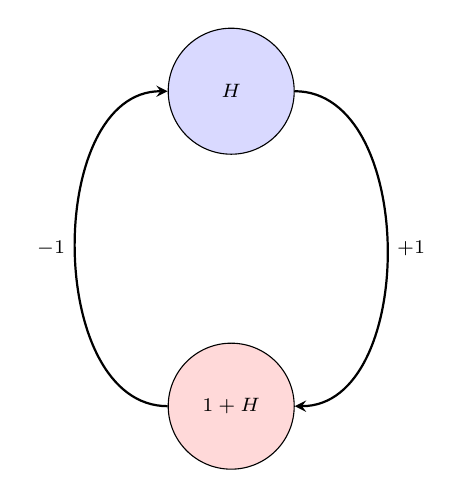
\begin{tikzpicture}[>=stealth, scale=2]
        \tikzset{
            num/.style={circle,draw,inner sep=4pt, minimum size=16mm},
            odd/.style={fill=red!15},
            even/.style={fill=blue!15}
        }
    
        \node[num,even]  (A) at (0,1) {\scriptsize$H$};
        \node[num,odd] (B) at ( 0,-1) {\scriptsize$1+H$};
    
        \draw[->,thick,bend left=90, black] (B) to node[left] {\scriptsize$-1$} (A);
        \draw[->,thick,bend left=90, black] (A) to node[right] {\scriptsize$+1$} (B);
        \end{tikzpicture}
        \captionof{figure}{Movement between the cosets for even $n$.}
\end{minipage}

\begin{minipage}[t]{0.6\textwidth}
\raggedright
\vfill
\textbf{However, when $n$ is odd}, the subset $H$ no longer forms a subgroup of $\mathbb{Z}_n$. Since $H$ is not a subgroup it has no cosets that partition $\mathbb{Z}_n$ and this parity breaks. \\
Wrapping around connects an even node to another even node, breaking the even-odd separation. Since this step links even and even residues, the parity between steps and position breaks.
\vfill
\end{minipage}\hfill
\begin{minipage}[t]{0.35\textwidth}
\begin{figure}
    \begin{tikzpicture}[>=stealth]
    \tikzset{
        num/.style={circle,draw,inner sep=4pt, minimum size=12mm},
        odd/.style={fill=red!15},
        even/.style={fill=blue!15}
    }
   
    \node[num,even]  (A) at (-6,0) {\scriptsize$0$};
    \node[num,odd] (B) at (-4,0) {\scriptsize$1$};
    \node[num,even]  (C) at (-2,0) {\scriptsize$2$};
    \node[num,odd] (D) at ( 0,0) {\scriptsize$3$};
    \node[num,even] (E) at ( 2,0) {\scriptsize$4$};
   
    \draw[->,thick,blue!70!black] ($(A.east)+(0,+0.1)$) -- ($(B.west)+(0,+0.1)$);
    \draw[->,thick,blue!70!black] ($(C.east)+(0,+0.1)$) -- ($(D.west)+(0,+0.1)$);
   
    \draw[->,thick,red!70!black]  ($(B.west)+(0,-0.1)$) -- ($(A.east)+(0,-0.1)$);
    \draw[->,thick,red!70!black]  ($(D.west)+(0,-0.1)$) -- ($(C.east)+(0,-0.1)$);
    
    \draw[->,thick,blue!70!black] ($(B.east)+(0,+0.1)$) -- ($(C.west)+(0,+0.1)$);
    \draw[->,thick,blue!70!black] ($(D.east)+(0,+0.1)$) -- ($(E.west)+(0,+0.1)$);
    \draw[->,thick,red!70!black]  ($(C.west)+(0,-0.1)$) -- ($(B.east)+(0,-0.1)$);
    \draw[->,thick,red!70!black]  ($(E.west)+(0,-0.1)$) -- ($(D.east)+(0,-0.1)$);

    \draw[->,thick,bend left=30, blue!70!black] (E) to node[above] {} (A);
    \draw[->,thick,bend left=30, blue!70!black] (A) to node[below] {} (E);
    \end{tikzpicture}
    \caption{Break in parity of the random walk on $\mathbb{Z}_5$.}
\end{figure}
\end{minipage}







    

    